% Created by tikzDevice version 0.12 on 2019-02-01 15:24:19
% !TEX encoding = UTF-8 Unicode
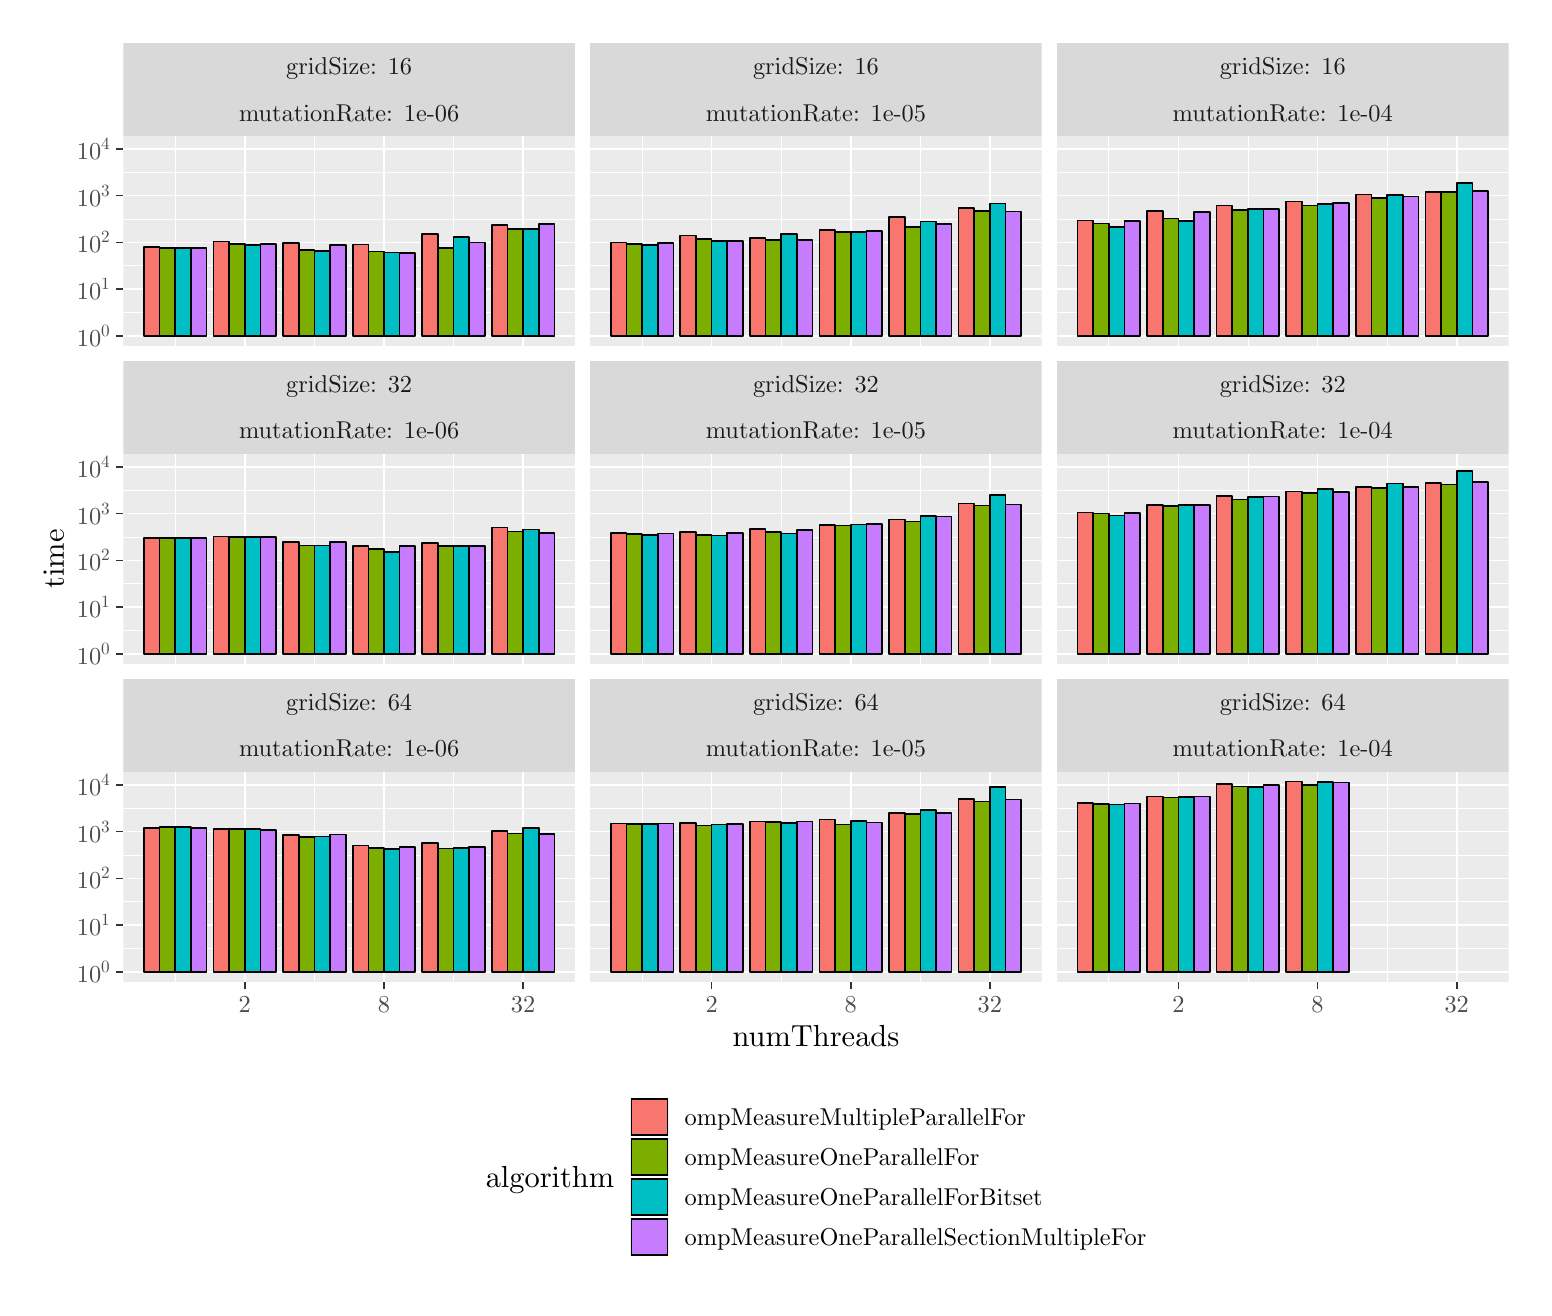
\begin{tikzpicture}[x=1pt,y=1pt]
\definecolor{fillColor}{RGB}{255,255,255}
\path[use as bounding box,fill=fillColor,fill opacity=0.00] (0,0) rectangle (540.60,455.24);
\begin{scope}
\path[clip] (  0.00,  0.00) rectangle (540.60,455.24);
\definecolor{drawColor}{RGB}{255,255,255}
\definecolor{fillColor}{RGB}{255,255,255}

\path[draw=drawColor,line width= 0.6pt,line join=round,line cap=round,fill=fillColor] (  0.00,  0.00) rectangle (540.60,455.24);
\end{scope}
\begin{scope}
\path[clip] ( 34.60,340.34) rectangle (197.77,416.13);
\definecolor{fillColor}{gray}{0.92}

\path[fill=fillColor] ( 34.60,340.34) rectangle (197.77,416.13);
\definecolor{drawColor}{RGB}{255,255,255}

\path[draw=drawColor,line width= 0.3pt,line join=round] ( 34.60,352.25) --
	(197.77,352.25);

\path[draw=drawColor,line width= 0.3pt,line join=round] ( 34.60,369.17) --
	(197.77,369.17);

\path[draw=drawColor,line width= 0.3pt,line join=round] ( 34.60,386.09) --
	(197.77,386.09);

\path[draw=drawColor,line width= 0.3pt,line join=round] ( 34.60,403.00) --
	(197.77,403.00);

\path[draw=drawColor,line width= 0.3pt,line join=round] ( 53.33,340.34) --
	( 53.33,416.13);

\path[draw=drawColor,line width= 0.3pt,line join=round] (103.61,340.34) --
	(103.61,416.13);

\path[draw=drawColor,line width= 0.3pt,line join=round] (153.89,340.34) --
	(153.89,416.13);

\path[draw=drawColor,line width= 0.6pt,line join=round] ( 34.60,343.79) --
	(197.77,343.79);

\path[draw=drawColor,line width= 0.6pt,line join=round] ( 34.60,360.71) --
	(197.77,360.71);

\path[draw=drawColor,line width= 0.6pt,line join=round] ( 34.60,377.63) --
	(197.77,377.63);

\path[draw=drawColor,line width= 0.6pt,line join=round] ( 34.60,394.55) --
	(197.77,394.55);

\path[draw=drawColor,line width= 0.6pt,line join=round] ( 34.60,411.46) --
	(197.77,411.46);

\path[draw=drawColor,line width= 0.6pt,line join=round] ( 78.47,340.34) --
	( 78.47,416.13);

\path[draw=drawColor,line width= 0.6pt,line join=round] (128.75,340.34) --
	(128.75,416.13);

\path[draw=drawColor,line width= 0.6pt,line join=round] (179.04,340.34) --
	(179.04,416.13);
\definecolor{drawColor}{RGB}{0,0,0}
\definecolor{fillColor}{RGB}{199,124,255}

\path[draw=drawColor,line width= 0.6pt,line join=round,fill=fillColor] ( 58.98,343.79) rectangle ( 64.64,375.73);
\definecolor{fillColor}{RGB}{0,191,196}

\path[draw=drawColor,line width= 0.6pt,line join=round,fill=fillColor] ( 53.33,343.79) rectangle ( 58.98,375.69);
\definecolor{fillColor}{RGB}{124,174,0}

\path[draw=drawColor,line width= 0.6pt,line join=round,fill=fillColor] ( 47.67,343.79) rectangle ( 53.33,375.66);
\definecolor{fillColor}{RGB}{248,118,109}

\path[draw=drawColor,line width= 0.6pt,line join=round,fill=fillColor] ( 42.01,343.79) rectangle ( 47.67,375.90);
\definecolor{fillColor}{RGB}{199,124,255}

\path[draw=drawColor,line width= 0.6pt,line join=round,fill=fillColor] ( 84.13,343.79) rectangle ( 89.78,377.08);
\definecolor{fillColor}{RGB}{0,191,196}

\path[draw=drawColor,line width= 0.6pt,line join=round,fill=fillColor] ( 78.47,343.79) rectangle ( 84.13,376.68);
\definecolor{fillColor}{RGB}{124,174,0}

\path[draw=drawColor,line width= 0.6pt,line join=round,fill=fillColor] ( 72.81,343.79) rectangle ( 78.47,377.10);
\definecolor{fillColor}{RGB}{248,118,109}

\path[draw=drawColor,line width= 0.6pt,line join=round,fill=fillColor] ( 67.16,343.79) rectangle ( 72.81,377.95);
\definecolor{fillColor}{RGB}{199,124,255}

\path[draw=drawColor,line width= 0.6pt,line join=round,fill=fillColor] (109.27,343.79) rectangle (114.92,376.61);
\definecolor{fillColor}{RGB}{0,191,196}

\path[draw=drawColor,line width= 0.6pt,line join=round,fill=fillColor] (103.61,343.79) rectangle (109.27,374.49);
\definecolor{fillColor}{RGB}{124,174,0}

\path[draw=drawColor,line width= 0.6pt,line join=round,fill=fillColor] ( 97.95,343.79) rectangle (103.61,374.89);
\definecolor{fillColor}{RGB}{248,118,109}

\path[draw=drawColor,line width= 0.6pt,line join=round,fill=fillColor] ( 92.30,343.79) rectangle ( 97.95,377.52);
\definecolor{fillColor}{RGB}{199,124,255}

\path[draw=drawColor,line width= 0.6pt,line join=round,fill=fillColor] (134.41,343.79) rectangle (140.07,373.87);
\definecolor{fillColor}{RGB}{0,191,196}

\path[draw=drawColor,line width= 0.6pt,line join=round,fill=fillColor] (128.75,343.79) rectangle (134.41,374.01);
\definecolor{fillColor}{RGB}{124,174,0}

\path[draw=drawColor,line width= 0.6pt,line join=round,fill=fillColor] (123.10,343.79) rectangle (128.75,374.40);
\definecolor{fillColor}{RGB}{248,118,109}

\path[draw=drawColor,line width= 0.6pt,line join=round,fill=fillColor] (117.44,343.79) rectangle (123.10,376.84);
\definecolor{fillColor}{RGB}{199,124,255}

\path[draw=drawColor,line width= 0.6pt,line join=round,fill=fillColor] (159.55,343.79) rectangle (165.21,377.57);
\definecolor{fillColor}{RGB}{0,191,196}

\path[draw=drawColor,line width= 0.6pt,line join=round,fill=fillColor] (153.89,343.79) rectangle (159.55,379.55);
\definecolor{fillColor}{RGB}{124,174,0}

\path[draw=drawColor,line width= 0.6pt,line join=round,fill=fillColor] (148.24,343.79) rectangle (153.89,375.61);
\definecolor{fillColor}{RGB}{248,118,109}

\path[draw=drawColor,line width= 0.6pt,line join=round,fill=fillColor] (142.58,343.79) rectangle (148.24,380.67);
\definecolor{fillColor}{RGB}{199,124,255}

\path[draw=drawColor,line width= 0.6pt,line join=round,fill=fillColor] (184.69,343.79) rectangle (190.35,384.38);
\definecolor{fillColor}{RGB}{0,191,196}

\path[draw=drawColor,line width= 0.6pt,line join=round,fill=fillColor] (179.04,343.79) rectangle (184.69,382.37);
\definecolor{fillColor}{RGB}{124,174,0}

\path[draw=drawColor,line width= 0.6pt,line join=round,fill=fillColor] (173.38,343.79) rectangle (179.04,382.54);
\definecolor{fillColor}{RGB}{248,118,109}

\path[draw=drawColor,line width= 0.6pt,line join=round,fill=fillColor] (167.72,343.79) rectangle (173.38,383.98);
\end{scope}
\begin{scope}
\path[clip] ( 34.60,225.44) rectangle (197.77,301.23);
\definecolor{fillColor}{gray}{0.92}

\path[fill=fillColor] ( 34.60,225.44) rectangle (197.77,301.23);
\definecolor{drawColor}{RGB}{255,255,255}

\path[draw=drawColor,line width= 0.3pt,line join=round] ( 34.60,237.35) --
	(197.77,237.35);

\path[draw=drawColor,line width= 0.3pt,line join=round] ( 34.60,254.27) --
	(197.77,254.27);

\path[draw=drawColor,line width= 0.3pt,line join=round] ( 34.60,271.18) --
	(197.77,271.18);

\path[draw=drawColor,line width= 0.3pt,line join=round] ( 34.60,288.10) --
	(197.77,288.10);

\path[draw=drawColor,line width= 0.3pt,line join=round] ( 53.33,225.44) --
	( 53.33,301.23);

\path[draw=drawColor,line width= 0.3pt,line join=round] (103.61,225.44) --
	(103.61,301.23);

\path[draw=drawColor,line width= 0.3pt,line join=round] (153.89,225.44) --
	(153.89,301.23);

\path[draw=drawColor,line width= 0.6pt,line join=round] ( 34.60,228.89) --
	(197.77,228.89);

\path[draw=drawColor,line width= 0.6pt,line join=round] ( 34.60,245.81) --
	(197.77,245.81);

\path[draw=drawColor,line width= 0.6pt,line join=round] ( 34.60,262.72) --
	(197.77,262.72);

\path[draw=drawColor,line width= 0.6pt,line join=round] ( 34.60,279.64) --
	(197.77,279.64);

\path[draw=drawColor,line width= 0.6pt,line join=round] ( 34.60,296.56) --
	(197.77,296.56);

\path[draw=drawColor,line width= 0.6pt,line join=round] ( 78.47,225.44) --
	( 78.47,301.23);

\path[draw=drawColor,line width= 0.6pt,line join=round] (128.75,225.44) --
	(128.75,301.23);

\path[draw=drawColor,line width= 0.6pt,line join=round] (179.04,225.44) --
	(179.04,301.23);
\definecolor{drawColor}{RGB}{0,0,0}
\definecolor{fillColor}{RGB}{199,124,255}

\path[draw=drawColor,line width= 0.6pt,line join=round,fill=fillColor] ( 58.98,228.89) rectangle ( 64.64,270.80);
\definecolor{fillColor}{RGB}{0,191,196}

\path[draw=drawColor,line width= 0.6pt,line join=round,fill=fillColor] ( 53.33,228.89) rectangle ( 58.98,270.89);
\definecolor{fillColor}{RGB}{124,174,0}

\path[draw=drawColor,line width= 0.6pt,line join=round,fill=fillColor] ( 47.67,228.89) rectangle ( 53.33,270.94);
\definecolor{fillColor}{RGB}{248,118,109}

\path[draw=drawColor,line width= 0.6pt,line join=round,fill=fillColor] ( 42.01,228.89) rectangle ( 47.67,270.90);
\definecolor{fillColor}{RGB}{199,124,255}

\path[draw=drawColor,line width= 0.6pt,line join=round,fill=fillColor] ( 84.13,228.89) rectangle ( 89.78,271.18);
\definecolor{fillColor}{RGB}{0,191,196}

\path[draw=drawColor,line width= 0.6pt,line join=round,fill=fillColor] ( 78.47,228.89) rectangle ( 84.13,271.19);
\definecolor{fillColor}{RGB}{124,174,0}

\path[draw=drawColor,line width= 0.6pt,line join=round,fill=fillColor] ( 72.81,228.89) rectangle ( 78.47,271.29);
\definecolor{fillColor}{RGB}{248,118,109}

\path[draw=drawColor,line width= 0.6pt,line join=round,fill=fillColor] ( 67.16,228.89) rectangle ( 72.81,271.35);
\definecolor{fillColor}{RGB}{199,124,255}

\path[draw=drawColor,line width= 0.6pt,line join=round,fill=fillColor] (109.27,228.89) rectangle (114.92,269.39);
\definecolor{fillColor}{RGB}{0,191,196}

\path[draw=drawColor,line width= 0.6pt,line join=round,fill=fillColor] (103.61,228.89) rectangle (109.27,268.09);
\definecolor{fillColor}{RGB}{124,174,0}

\path[draw=drawColor,line width= 0.6pt,line join=round,fill=fillColor] ( 97.95,228.89) rectangle (103.61,268.13);
\definecolor{fillColor}{RGB}{248,118,109}

\path[draw=drawColor,line width= 0.6pt,line join=round,fill=fillColor] ( 92.30,228.89) rectangle ( 97.95,269.30);
\definecolor{fillColor}{RGB}{199,124,255}

\path[draw=drawColor,line width= 0.6pt,line join=round,fill=fillColor] (134.41,228.89) rectangle (140.07,267.89);
\definecolor{fillColor}{RGB}{0,191,196}

\path[draw=drawColor,line width= 0.6pt,line join=round,fill=fillColor] (128.75,228.89) rectangle (134.41,265.79);
\definecolor{fillColor}{RGB}{124,174,0}

\path[draw=drawColor,line width= 0.6pt,line join=round,fill=fillColor] (123.10,228.89) rectangle (128.75,266.81);
\definecolor{fillColor}{RGB}{248,118,109}

\path[draw=drawColor,line width= 0.6pt,line join=round,fill=fillColor] (117.44,228.89) rectangle (123.10,267.96);
\definecolor{fillColor}{RGB}{199,124,255}

\path[draw=drawColor,line width= 0.6pt,line join=round,fill=fillColor] (159.55,228.89) rectangle (165.21,267.83);
\definecolor{fillColor}{RGB}{0,191,196}

\path[draw=drawColor,line width= 0.6pt,line join=round,fill=fillColor] (153.89,228.89) rectangle (159.55,267.92);
\definecolor{fillColor}{RGB}{124,174,0}

\path[draw=drawColor,line width= 0.6pt,line join=round,fill=fillColor] (148.24,228.89) rectangle (153.89,267.96);
\definecolor{fillColor}{RGB}{248,118,109}

\path[draw=drawColor,line width= 0.6pt,line join=round,fill=fillColor] (142.58,228.89) rectangle (148.24,269.10);
\definecolor{fillColor}{RGB}{199,124,255}

\path[draw=drawColor,line width= 0.6pt,line join=round,fill=fillColor] (184.69,228.89) rectangle (190.35,272.71);
\definecolor{fillColor}{RGB}{0,191,196}

\path[draw=drawColor,line width= 0.6pt,line join=round,fill=fillColor] (179.04,228.89) rectangle (184.69,273.95);
\definecolor{fillColor}{RGB}{124,174,0}

\path[draw=drawColor,line width= 0.6pt,line join=round,fill=fillColor] (173.38,228.89) rectangle (179.04,273.12);
\definecolor{fillColor}{RGB}{248,118,109}

\path[draw=drawColor,line width= 0.6pt,line join=round,fill=fillColor] (167.72,228.89) rectangle (173.38,274.58);
\end{scope}
\begin{scope}
\path[clip] ( 34.60,110.54) rectangle (197.77,186.33);
\definecolor{fillColor}{gray}{0.92}

\path[fill=fillColor] ( 34.60,110.54) rectangle (197.77,186.33);
\definecolor{drawColor}{RGB}{255,255,255}

\path[draw=drawColor,line width= 0.3pt,line join=round] ( 34.60,122.45) --
	(197.77,122.45);

\path[draw=drawColor,line width= 0.3pt,line join=round] ( 34.60,139.36) --
	(197.77,139.36);

\path[draw=drawColor,line width= 0.3pt,line join=round] ( 34.60,156.28) --
	(197.77,156.28);

\path[draw=drawColor,line width= 0.3pt,line join=round] ( 34.60,173.20) --
	(197.77,173.20);

\path[draw=drawColor,line width= 0.3pt,line join=round] ( 53.33,110.54) --
	( 53.33,186.33);

\path[draw=drawColor,line width= 0.3pt,line join=round] (103.61,110.54) --
	(103.61,186.33);

\path[draw=drawColor,line width= 0.3pt,line join=round] (153.89,110.54) --
	(153.89,186.33);

\path[draw=drawColor,line width= 0.6pt,line join=round] ( 34.60,113.99) --
	(197.77,113.99);

\path[draw=drawColor,line width= 0.6pt,line join=round] ( 34.60,130.90) --
	(197.77,130.90);

\path[draw=drawColor,line width= 0.6pt,line join=round] ( 34.60,147.82) --
	(197.77,147.82);

\path[draw=drawColor,line width= 0.6pt,line join=round] ( 34.60,164.74) --
	(197.77,164.74);

\path[draw=drawColor,line width= 0.6pt,line join=round] ( 34.60,181.66) --
	(197.77,181.66);

\path[draw=drawColor,line width= 0.6pt,line join=round] ( 78.47,110.54) --
	( 78.47,186.33);

\path[draw=drawColor,line width= 0.6pt,line join=round] (128.75,110.54) --
	(128.75,186.33);

\path[draw=drawColor,line width= 0.6pt,line join=round] (179.04,110.54) --
	(179.04,186.33);
\definecolor{drawColor}{RGB}{0,0,0}
\definecolor{fillColor}{RGB}{199,124,255}

\path[draw=drawColor,line width= 0.6pt,line join=round,fill=fillColor] ( 58.98,113.99) rectangle ( 64.64,166.09);
\definecolor{fillColor}{RGB}{0,191,196}

\path[draw=drawColor,line width= 0.6pt,line join=round,fill=fillColor] ( 53.33,113.99) rectangle ( 58.98,166.31);
\definecolor{fillColor}{RGB}{124,174,0}

\path[draw=drawColor,line width= 0.6pt,line join=round,fill=fillColor] ( 47.67,113.99) rectangle ( 53.33,166.29);
\definecolor{fillColor}{RGB}{248,118,109}

\path[draw=drawColor,line width= 0.6pt,line join=round,fill=fillColor] ( 42.01,113.99) rectangle ( 47.67,166.14);
\definecolor{fillColor}{RGB}{199,124,255}

\path[draw=drawColor,line width= 0.6pt,line join=round,fill=fillColor] ( 84.13,113.99) rectangle ( 89.78,165.41);
\definecolor{fillColor}{RGB}{0,191,196}

\path[draw=drawColor,line width= 0.6pt,line join=round,fill=fillColor] ( 78.47,113.99) rectangle ( 84.13,165.57);
\definecolor{fillColor}{RGB}{124,174,0}

\path[draw=drawColor,line width= 0.6pt,line join=round,fill=fillColor] ( 72.81,113.99) rectangle ( 78.47,165.62);
\definecolor{fillColor}{RGB}{248,118,109}

\path[draw=drawColor,line width= 0.6pt,line join=round,fill=fillColor] ( 67.16,113.99) rectangle ( 72.81,165.63);
\definecolor{fillColor}{RGB}{199,124,255}

\path[draw=drawColor,line width= 0.6pt,line join=round,fill=fillColor] (109.27,113.99) rectangle (114.92,163.65);
\definecolor{fillColor}{RGB}{0,191,196}

\path[draw=drawColor,line width= 0.6pt,line join=round,fill=fillColor] (103.61,113.99) rectangle (109.27,162.93);
\definecolor{fillColor}{RGB}{124,174,0}

\path[draw=drawColor,line width= 0.6pt,line join=round,fill=fillColor] ( 97.95,113.99) rectangle (103.61,162.88);
\definecolor{fillColor}{RGB}{248,118,109}

\path[draw=drawColor,line width= 0.6pt,line join=round,fill=fillColor] ( 92.30,113.99) rectangle ( 97.95,163.62);
\definecolor{fillColor}{RGB}{199,124,255}

\path[draw=drawColor,line width= 0.6pt,line join=round,fill=fillColor] (134.41,113.99) rectangle (140.07,159.13);
\definecolor{fillColor}{RGB}{0,191,196}

\path[draw=drawColor,line width= 0.6pt,line join=round,fill=fillColor] (128.75,113.99) rectangle (134.41,158.46);
\definecolor{fillColor}{RGB}{124,174,0}

\path[draw=drawColor,line width= 0.6pt,line join=round,fill=fillColor] (123.10,113.99) rectangle (128.75,158.91);
\definecolor{fillColor}{RGB}{248,118,109}

\path[draw=drawColor,line width= 0.6pt,line join=round,fill=fillColor] (117.44,113.99) rectangle (123.10,159.74);
\definecolor{fillColor}{RGB}{199,124,255}

\path[draw=drawColor,line width= 0.6pt,line join=round,fill=fillColor] (159.55,113.99) rectangle (165.21,159.18);
\definecolor{fillColor}{RGB}{0,191,196}

\path[draw=drawColor,line width= 0.6pt,line join=round,fill=fillColor] (153.89,113.99) rectangle (159.55,158.77);
\definecolor{fillColor}{RGB}{124,174,0}

\path[draw=drawColor,line width= 0.6pt,line join=round,fill=fillColor] (148.24,113.99) rectangle (153.89,158.61);
\definecolor{fillColor}{RGB}{248,118,109}

\path[draw=drawColor,line width= 0.6pt,line join=round,fill=fillColor] (142.58,113.99) rectangle (148.24,160.52);
\definecolor{fillColor}{RGB}{199,124,255}

\path[draw=drawColor,line width= 0.6pt,line join=round,fill=fillColor] (184.69,113.99) rectangle (190.35,163.92);
\definecolor{fillColor}{RGB}{0,191,196}

\path[draw=drawColor,line width= 0.6pt,line join=round,fill=fillColor] (179.04,113.99) rectangle (184.69,166.02);
\definecolor{fillColor}{RGB}{124,174,0}

\path[draw=drawColor,line width= 0.6pt,line join=round,fill=fillColor] (173.38,113.99) rectangle (179.04,164.08);
\definecolor{fillColor}{RGB}{248,118,109}

\path[draw=drawColor,line width= 0.6pt,line join=round,fill=fillColor] (167.72,113.99) rectangle (173.38,164.87);
\end{scope}
\begin{scope}
\path[clip] (203.27,340.34) rectangle (366.43,416.13);
\definecolor{fillColor}{gray}{0.92}

\path[fill=fillColor] (203.27,340.34) rectangle (366.43,416.13);
\definecolor{drawColor}{RGB}{255,255,255}

\path[draw=drawColor,line width= 0.3pt,line join=round] (203.27,352.25) --
	(366.43,352.25);

\path[draw=drawColor,line width= 0.3pt,line join=round] (203.27,369.17) --
	(366.43,369.17);

\path[draw=drawColor,line width= 0.3pt,line join=round] (203.27,386.09) --
	(366.43,386.09);

\path[draw=drawColor,line width= 0.3pt,line join=round] (203.27,403.00) --
	(366.43,403.00);

\path[draw=drawColor,line width= 0.3pt,line join=round] (222.00,340.34) --
	(222.00,416.13);

\path[draw=drawColor,line width= 0.3pt,line join=round] (272.28,340.34) --
	(272.28,416.13);

\path[draw=drawColor,line width= 0.3pt,line join=round] (322.56,340.34) --
	(322.56,416.13);

\path[draw=drawColor,line width= 0.6pt,line join=round] (203.27,343.79) --
	(366.43,343.79);

\path[draw=drawColor,line width= 0.6pt,line join=round] (203.27,360.71) --
	(366.43,360.71);

\path[draw=drawColor,line width= 0.6pt,line join=round] (203.27,377.63) --
	(366.43,377.63);

\path[draw=drawColor,line width= 0.6pt,line join=round] (203.27,394.55) --
	(366.43,394.55);

\path[draw=drawColor,line width= 0.6pt,line join=round] (203.27,411.46) --
	(366.43,411.46);

\path[draw=drawColor,line width= 0.6pt,line join=round] (247.14,340.34) --
	(247.14,416.13);

\path[draw=drawColor,line width= 0.6pt,line join=round] (297.42,340.34) --
	(297.42,416.13);

\path[draw=drawColor,line width= 0.6pt,line join=round] (347.70,340.34) --
	(347.70,416.13);
\definecolor{drawColor}{RGB}{0,0,0}
\definecolor{fillColor}{RGB}{199,124,255}

\path[draw=drawColor,line width= 0.6pt,line join=round,fill=fillColor] (227.65,343.79) rectangle (233.31,377.51);
\definecolor{fillColor}{RGB}{0,191,196}

\path[draw=drawColor,line width= 0.6pt,line join=round,fill=fillColor] (222.00,343.79) rectangle (227.65,376.73);
\definecolor{fillColor}{RGB}{124,174,0}

\path[draw=drawColor,line width= 0.6pt,line join=round,fill=fillColor] (216.34,343.79) rectangle (222.00,377.14);
\definecolor{fillColor}{RGB}{248,118,109}

\path[draw=drawColor,line width= 0.6pt,line join=round,fill=fillColor] (210.68,343.79) rectangle (216.34,377.56);
\definecolor{fillColor}{RGB}{199,124,255}

\path[draw=drawColor,line width= 0.6pt,line join=round,fill=fillColor] (252.79,343.79) rectangle (258.45,378.19);
\definecolor{fillColor}{RGB}{0,191,196}

\path[draw=drawColor,line width= 0.6pt,line join=round,fill=fillColor] (247.14,343.79) rectangle (252.79,378.15);
\definecolor{fillColor}{RGB}{124,174,0}

\path[draw=drawColor,line width= 0.6pt,line join=round,fill=fillColor] (241.48,343.79) rectangle (247.14,378.86);
\definecolor{fillColor}{RGB}{248,118,109}

\path[draw=drawColor,line width= 0.6pt,line join=round,fill=fillColor] (235.82,343.79) rectangle (241.48,380.16);
\definecolor{fillColor}{RGB}{199,124,255}

\path[draw=drawColor,line width= 0.6pt,line join=round,fill=fillColor] (277.94,343.79) rectangle (283.59,378.48);
\definecolor{fillColor}{RGB}{0,191,196}

\path[draw=drawColor,line width= 0.6pt,line join=round,fill=fillColor] (272.28,343.79) rectangle (277.94,380.71);
\definecolor{fillColor}{RGB}{124,174,0}

\path[draw=drawColor,line width= 0.6pt,line join=round,fill=fillColor] (266.62,343.79) rectangle (272.28,378.41);
\definecolor{fillColor}{RGB}{248,118,109}

\path[draw=drawColor,line width= 0.6pt,line join=round,fill=fillColor] (260.97,343.79) rectangle (266.62,379.32);
\definecolor{fillColor}{RGB}{199,124,255}

\path[draw=drawColor,line width= 0.6pt,line join=round,fill=fillColor] (303.08,343.79) rectangle (308.73,381.69);
\definecolor{fillColor}{RGB}{0,191,196}

\path[draw=drawColor,line width= 0.6pt,line join=round,fill=fillColor] (297.42,343.79) rectangle (303.08,381.40);
\definecolor{fillColor}{RGB}{124,174,0}

\path[draw=drawColor,line width= 0.6pt,line join=round,fill=fillColor] (291.76,343.79) rectangle (297.42,381.39);
\definecolor{fillColor}{RGB}{248,118,109}

\path[draw=drawColor,line width= 0.6pt,line join=round,fill=fillColor] (286.11,343.79) rectangle (291.76,382.11);
\definecolor{fillColor}{RGB}{199,124,255}

\path[draw=drawColor,line width= 0.6pt,line join=round,fill=fillColor] (328.22,343.79) rectangle (333.88,384.25);
\definecolor{fillColor}{RGB}{0,191,196}

\path[draw=drawColor,line width= 0.6pt,line join=round,fill=fillColor] (322.56,343.79) rectangle (328.22,385.24);
\definecolor{fillColor}{RGB}{124,174,0}

\path[draw=drawColor,line width= 0.6pt,line join=round,fill=fillColor] (316.91,343.79) rectangle (322.56,383.29);
\definecolor{fillColor}{RGB}{248,118,109}

\path[draw=drawColor,line width= 0.6pt,line join=round,fill=fillColor] (311.25,343.79) rectangle (316.91,386.93);
\definecolor{fillColor}{RGB}{199,124,255}

\path[draw=drawColor,line width= 0.6pt,line join=round,fill=fillColor] (353.36,343.79) rectangle (359.02,388.83);
\definecolor{fillColor}{RGB}{0,191,196}

\path[draw=drawColor,line width= 0.6pt,line join=round,fill=fillColor] (347.70,343.79) rectangle (353.36,391.73);
\definecolor{fillColor}{RGB}{124,174,0}

\path[draw=drawColor,line width= 0.6pt,line join=round,fill=fillColor] (342.05,343.79) rectangle (347.70,388.90);
\definecolor{fillColor}{RGB}{248,118,109}

\path[draw=drawColor,line width= 0.6pt,line join=round,fill=fillColor] (336.39,343.79) rectangle (342.05,390.03);
\end{scope}
\begin{scope}
\path[clip] (203.27,225.44) rectangle (366.43,301.23);
\definecolor{fillColor}{gray}{0.92}

\path[fill=fillColor] (203.27,225.44) rectangle (366.43,301.23);
\definecolor{drawColor}{RGB}{255,255,255}

\path[draw=drawColor,line width= 0.3pt,line join=round] (203.27,237.35) --
	(366.43,237.35);

\path[draw=drawColor,line width= 0.3pt,line join=round] (203.27,254.27) --
	(366.43,254.27);

\path[draw=drawColor,line width= 0.3pt,line join=round] (203.27,271.18) --
	(366.43,271.18);

\path[draw=drawColor,line width= 0.3pt,line join=round] (203.27,288.10) --
	(366.43,288.10);

\path[draw=drawColor,line width= 0.3pt,line join=round] (222.00,225.44) --
	(222.00,301.23);

\path[draw=drawColor,line width= 0.3pt,line join=round] (272.28,225.44) --
	(272.28,301.23);

\path[draw=drawColor,line width= 0.3pt,line join=round] (322.56,225.44) --
	(322.56,301.23);

\path[draw=drawColor,line width= 0.6pt,line join=round] (203.27,228.89) --
	(366.43,228.89);

\path[draw=drawColor,line width= 0.6pt,line join=round] (203.27,245.81) --
	(366.43,245.81);

\path[draw=drawColor,line width= 0.6pt,line join=round] (203.27,262.72) --
	(366.43,262.72);

\path[draw=drawColor,line width= 0.6pt,line join=round] (203.27,279.64) --
	(366.43,279.64);

\path[draw=drawColor,line width= 0.6pt,line join=round] (203.27,296.56) --
	(366.43,296.56);

\path[draw=drawColor,line width= 0.6pt,line join=round] (247.14,225.44) --
	(247.14,301.23);

\path[draw=drawColor,line width= 0.6pt,line join=round] (297.42,225.44) --
	(297.42,301.23);

\path[draw=drawColor,line width= 0.6pt,line join=round] (347.70,225.44) --
	(347.70,301.23);
\definecolor{drawColor}{RGB}{0,0,0}
\definecolor{fillColor}{RGB}{199,124,255}

\path[draw=drawColor,line width= 0.6pt,line join=round,fill=fillColor] (227.65,228.89) rectangle (233.31,272.40);
\definecolor{fillColor}{RGB}{0,191,196}

\path[draw=drawColor,line width= 0.6pt,line join=round,fill=fillColor] (222.00,228.89) rectangle (227.65,271.90);
\definecolor{fillColor}{RGB}{124,174,0}

\path[draw=drawColor,line width= 0.6pt,line join=round,fill=fillColor] (216.34,228.89) rectangle (222.00,272.24);
\definecolor{fillColor}{RGB}{248,118,109}

\path[draw=drawColor,line width= 0.6pt,line join=round,fill=fillColor] (210.68,228.89) rectangle (216.34,272.52);
\definecolor{fillColor}{RGB}{199,124,255}

\path[draw=drawColor,line width= 0.6pt,line join=round,fill=fillColor] (252.79,228.89) rectangle (258.45,272.67);
\definecolor{fillColor}{RGB}{0,191,196}

\path[draw=drawColor,line width= 0.6pt,line join=round,fill=fillColor] (247.14,228.89) rectangle (252.79,271.73);
\definecolor{fillColor}{RGB}{124,174,0}

\path[draw=drawColor,line width= 0.6pt,line join=round,fill=fillColor] (241.48,228.89) rectangle (247.14,271.94);
\definecolor{fillColor}{RGB}{248,118,109}

\path[draw=drawColor,line width= 0.6pt,line join=round,fill=fillColor] (235.82,228.89) rectangle (241.48,272.90);
\definecolor{fillColor}{RGB}{199,124,255}

\path[draw=drawColor,line width= 0.6pt,line join=round,fill=fillColor] (277.94,228.89) rectangle (283.59,273.70);
\definecolor{fillColor}{RGB}{0,191,196}

\path[draw=drawColor,line width= 0.6pt,line join=round,fill=fillColor] (272.28,228.89) rectangle (277.94,272.51);
\definecolor{fillColor}{RGB}{124,174,0}

\path[draw=drawColor,line width= 0.6pt,line join=round,fill=fillColor] (266.62,228.89) rectangle (272.28,272.92);
\definecolor{fillColor}{RGB}{248,118,109}

\path[draw=drawColor,line width= 0.6pt,line join=round,fill=fillColor] (260.97,228.89) rectangle (266.62,274.06);
\definecolor{fillColor}{RGB}{199,124,255}

\path[draw=drawColor,line width= 0.6pt,line join=round,fill=fillColor] (303.08,228.89) rectangle (308.73,275.90);
\definecolor{fillColor}{RGB}{0,191,196}

\path[draw=drawColor,line width= 0.6pt,line join=round,fill=fillColor] (297.42,228.89) rectangle (303.08,275.67);
\definecolor{fillColor}{RGB}{124,174,0}

\path[draw=drawColor,line width= 0.6pt,line join=round,fill=fillColor] (291.76,228.89) rectangle (297.42,275.35);
\definecolor{fillColor}{RGB}{248,118,109}

\path[draw=drawColor,line width= 0.6pt,line join=round,fill=fillColor] (286.11,228.89) rectangle (291.76,275.42);
\definecolor{fillColor}{RGB}{199,124,255}

\path[draw=drawColor,line width= 0.6pt,line join=round,fill=fillColor] (328.22,228.89) rectangle (333.88,278.54);
\definecolor{fillColor}{RGB}{0,191,196}

\path[draw=drawColor,line width= 0.6pt,line join=round,fill=fillColor] (322.56,228.89) rectangle (328.22,278.74);
\definecolor{fillColor}{RGB}{124,174,0}

\path[draw=drawColor,line width= 0.6pt,line join=round,fill=fillColor] (316.91,228.89) rectangle (322.56,276.75);
\definecolor{fillColor}{RGB}{248,118,109}

\path[draw=drawColor,line width= 0.6pt,line join=round,fill=fillColor] (311.25,228.89) rectangle (316.91,277.54);
\definecolor{fillColor}{RGB}{199,124,255}

\path[draw=drawColor,line width= 0.6pt,line join=round,fill=fillColor] (353.36,228.89) rectangle (359.02,282.99);
\definecolor{fillColor}{RGB}{0,191,196}

\path[draw=drawColor,line width= 0.6pt,line join=round,fill=fillColor] (347.70,228.89) rectangle (353.36,286.31);
\definecolor{fillColor}{RGB}{124,174,0}

\path[draw=drawColor,line width= 0.6pt,line join=round,fill=fillColor] (342.05,228.89) rectangle (347.70,282.61);
\definecolor{fillColor}{RGB}{248,118,109}

\path[draw=drawColor,line width= 0.6pt,line join=round,fill=fillColor] (336.39,228.89) rectangle (342.05,283.33);
\end{scope}
\begin{scope}
\path[clip] (203.27,110.54) rectangle (366.43,186.33);
\definecolor{fillColor}{gray}{0.92}

\path[fill=fillColor] (203.27,110.54) rectangle (366.43,186.33);
\definecolor{drawColor}{RGB}{255,255,255}

\path[draw=drawColor,line width= 0.3pt,line join=round] (203.27,122.45) --
	(366.43,122.45);

\path[draw=drawColor,line width= 0.3pt,line join=round] (203.27,139.36) --
	(366.43,139.36);

\path[draw=drawColor,line width= 0.3pt,line join=round] (203.27,156.28) --
	(366.43,156.28);

\path[draw=drawColor,line width= 0.3pt,line join=round] (203.27,173.20) --
	(366.43,173.20);

\path[draw=drawColor,line width= 0.3pt,line join=round] (222.00,110.54) --
	(222.00,186.33);

\path[draw=drawColor,line width= 0.3pt,line join=round] (272.28,110.54) --
	(272.28,186.33);

\path[draw=drawColor,line width= 0.3pt,line join=round] (322.56,110.54) --
	(322.56,186.33);

\path[draw=drawColor,line width= 0.6pt,line join=round] (203.27,113.99) --
	(366.43,113.99);

\path[draw=drawColor,line width= 0.6pt,line join=round] (203.27,130.90) --
	(366.43,130.90);

\path[draw=drawColor,line width= 0.6pt,line join=round] (203.27,147.82) --
	(366.43,147.82);

\path[draw=drawColor,line width= 0.6pt,line join=round] (203.27,164.74) --
	(366.43,164.74);

\path[draw=drawColor,line width= 0.6pt,line join=round] (203.27,181.66) --
	(366.43,181.66);

\path[draw=drawColor,line width= 0.6pt,line join=round] (247.14,110.54) --
	(247.14,186.33);

\path[draw=drawColor,line width= 0.6pt,line join=round] (297.42,110.54) --
	(297.42,186.33);

\path[draw=drawColor,line width= 0.6pt,line join=round] (347.70,110.54) --
	(347.70,186.33);
\definecolor{drawColor}{RGB}{0,0,0}
\definecolor{fillColor}{RGB}{199,124,255}

\path[draw=drawColor,line width= 0.6pt,line join=round,fill=fillColor] (227.65,113.99) rectangle (233.31,167.65);
\definecolor{fillColor}{RGB}{0,191,196}

\path[draw=drawColor,line width= 0.6pt,line join=round,fill=fillColor] (222.00,113.99) rectangle (227.65,167.38);
\definecolor{fillColor}{RGB}{124,174,0}

\path[draw=drawColor,line width= 0.6pt,line join=round,fill=fillColor] (216.34,113.99) rectangle (222.00,167.60);
\definecolor{fillColor}{RGB}{248,118,109}

\path[draw=drawColor,line width= 0.6pt,line join=round,fill=fillColor] (210.68,113.99) rectangle (216.34,167.70);
\definecolor{fillColor}{RGB}{199,124,255}

\path[draw=drawColor,line width= 0.6pt,line join=round,fill=fillColor] (252.79,113.99) rectangle (258.45,167.58);
\definecolor{fillColor}{RGB}{0,191,196}

\path[draw=drawColor,line width= 0.6pt,line join=round,fill=fillColor] (247.14,113.99) rectangle (252.79,167.26);
\definecolor{fillColor}{RGB}{124,174,0}

\path[draw=drawColor,line width= 0.6pt,line join=round,fill=fillColor] (241.48,113.99) rectangle (247.14,166.96);
\definecolor{fillColor}{RGB}{248,118,109}

\path[draw=drawColor,line width= 0.6pt,line join=round,fill=fillColor] (235.82,113.99) rectangle (241.48,167.76);
\definecolor{fillColor}{RGB}{199,124,255}

\path[draw=drawColor,line width= 0.6pt,line join=round,fill=fillColor] (277.94,113.99) rectangle (283.59,168.43);
\definecolor{fillColor}{RGB}{0,191,196}

\path[draw=drawColor,line width= 0.6pt,line join=round,fill=fillColor] (272.28,113.99) rectangle (277.94,167.91);
\definecolor{fillColor}{RGB}{124,174,0}

\path[draw=drawColor,line width= 0.6pt,line join=round,fill=fillColor] (266.62,113.99) rectangle (272.28,168.12);
\definecolor{fillColor}{RGB}{248,118,109}

\path[draw=drawColor,line width= 0.6pt,line join=round,fill=fillColor] (260.97,113.99) rectangle (266.62,168.39);
\definecolor{fillColor}{RGB}{199,124,255}

\path[draw=drawColor,line width= 0.6pt,line join=round,fill=fillColor] (303.08,113.99) rectangle (308.73,167.99);
\definecolor{fillColor}{RGB}{0,191,196}

\path[draw=drawColor,line width= 0.6pt,line join=round,fill=fillColor] (297.42,113.99) rectangle (303.08,168.48);
\definecolor{fillColor}{RGB}{124,174,0}

\path[draw=drawColor,line width= 0.6pt,line join=round,fill=fillColor] (291.76,113.99) rectangle (297.42,167.28);
\definecolor{fillColor}{RGB}{248,118,109}

\path[draw=drawColor,line width= 0.6pt,line join=round,fill=fillColor] (286.11,113.99) rectangle (291.76,169.06);
\definecolor{fillColor}{RGB}{199,124,255}

\path[draw=drawColor,line width= 0.6pt,line join=round,fill=fillColor] (328.22,113.99) rectangle (333.88,171.54);
\definecolor{fillColor}{RGB}{0,191,196}

\path[draw=drawColor,line width= 0.6pt,line join=round,fill=fillColor] (322.56,113.99) rectangle (328.22,172.63);
\definecolor{fillColor}{RGB}{124,174,0}

\path[draw=drawColor,line width= 0.6pt,line join=round,fill=fillColor] (316.91,113.99) rectangle (322.56,171.04);
\definecolor{fillColor}{RGB}{248,118,109}

\path[draw=drawColor,line width= 0.6pt,line join=round,fill=fillColor] (311.25,113.99) rectangle (316.91,171.55);
\definecolor{fillColor}{RGB}{199,124,255}

\path[draw=drawColor,line width= 0.6pt,line join=round,fill=fillColor] (353.36,113.99) rectangle (359.02,176.33);
\definecolor{fillColor}{RGB}{0,191,196}

\path[draw=drawColor,line width= 0.6pt,line join=round,fill=fillColor] (347.70,113.99) rectangle (353.36,180.77);
\definecolor{fillColor}{RGB}{124,174,0}

\path[draw=drawColor,line width= 0.6pt,line join=round,fill=fillColor] (342.05,113.99) rectangle (347.70,175.56);
\definecolor{fillColor}{RGB}{248,118,109}

\path[draw=drawColor,line width= 0.6pt,line join=round,fill=fillColor] (336.39,113.99) rectangle (342.05,176.57);
\end{scope}
\begin{scope}
\path[clip] (371.93,340.34) rectangle (535.10,416.13);
\definecolor{fillColor}{gray}{0.92}

\path[fill=fillColor] (371.93,340.34) rectangle (535.10,416.13);
\definecolor{drawColor}{RGB}{255,255,255}

\path[draw=drawColor,line width= 0.3pt,line join=round] (371.93,352.25) --
	(535.10,352.25);

\path[draw=drawColor,line width= 0.3pt,line join=round] (371.93,369.17) --
	(535.10,369.17);

\path[draw=drawColor,line width= 0.3pt,line join=round] (371.93,386.09) --
	(535.10,386.09);

\path[draw=drawColor,line width= 0.3pt,line join=round] (371.93,403.00) --
	(535.10,403.00);

\path[draw=drawColor,line width= 0.3pt,line join=round] (390.66,340.34) --
	(390.66,416.13);

\path[draw=drawColor,line width= 0.3pt,line join=round] (440.95,340.34) --
	(440.95,416.13);

\path[draw=drawColor,line width= 0.3pt,line join=round] (491.23,340.34) --
	(491.23,416.13);

\path[draw=drawColor,line width= 0.6pt,line join=round] (371.93,343.79) --
	(535.10,343.79);

\path[draw=drawColor,line width= 0.6pt,line join=round] (371.93,360.71) --
	(535.10,360.71);

\path[draw=drawColor,line width= 0.6pt,line join=round] (371.93,377.63) --
	(535.10,377.63);

\path[draw=drawColor,line width= 0.6pt,line join=round] (371.93,394.55) --
	(535.10,394.55);

\path[draw=drawColor,line width= 0.6pt,line join=round] (371.93,411.46) --
	(535.10,411.46);

\path[draw=drawColor,line width= 0.6pt,line join=round] (415.81,340.34) --
	(415.81,416.13);

\path[draw=drawColor,line width= 0.6pt,line join=round] (466.09,340.34) --
	(466.09,416.13);

\path[draw=drawColor,line width= 0.6pt,line join=round] (516.37,340.34) --
	(516.37,416.13);
\definecolor{drawColor}{RGB}{0,0,0}
\definecolor{fillColor}{RGB}{199,124,255}

\path[draw=drawColor,line width= 0.6pt,line join=round,fill=fillColor] (396.32,343.79) rectangle (401.98,385.42);
\definecolor{fillColor}{RGB}{0,191,196}

\path[draw=drawColor,line width= 0.6pt,line join=round,fill=fillColor] (390.66,343.79) rectangle (396.32,383.27);
\definecolor{fillColor}{RGB}{124,174,0}

\path[draw=drawColor,line width= 0.6pt,line join=round,fill=fillColor] (385.01,343.79) rectangle (390.66,384.43);
\definecolor{fillColor}{RGB}{248,118,109}

\path[draw=drawColor,line width= 0.6pt,line join=round,fill=fillColor] (379.35,343.79) rectangle (385.01,385.57);
\definecolor{fillColor}{RGB}{199,124,255}

\path[draw=drawColor,line width= 0.6pt,line join=round,fill=fillColor] (421.46,343.79) rectangle (427.12,388.59);
\definecolor{fillColor}{RGB}{0,191,196}

\path[draw=drawColor,line width= 0.6pt,line join=round,fill=fillColor] (415.81,343.79) rectangle (421.46,385.41);
\definecolor{fillColor}{RGB}{124,174,0}

\path[draw=drawColor,line width= 0.6pt,line join=round,fill=fillColor] (410.15,343.79) rectangle (415.81,386.31);
\definecolor{fillColor}{RGB}{248,118,109}

\path[draw=drawColor,line width= 0.6pt,line join=round,fill=fillColor] (404.49,343.79) rectangle (410.15,388.92);
\definecolor{fillColor}{RGB}{199,124,255}

\path[draw=drawColor,line width= 0.6pt,line join=round,fill=fillColor] (446.60,343.79) rectangle (452.26,389.80);
\definecolor{fillColor}{RGB}{0,191,196}

\path[draw=drawColor,line width= 0.6pt,line join=round,fill=fillColor] (440.95,343.79) rectangle (446.60,389.71);
\definecolor{fillColor}{RGB}{124,174,0}

\path[draw=drawColor,line width= 0.6pt,line join=round,fill=fillColor] (435.29,343.79) rectangle (440.95,389.36);
\definecolor{fillColor}{RGB}{248,118,109}

\path[draw=drawColor,line width= 0.6pt,line join=round,fill=fillColor] (429.63,343.79) rectangle (435.29,390.99);
\definecolor{fillColor}{RGB}{199,124,255}

\path[draw=drawColor,line width= 0.6pt,line join=round,fill=fillColor] (471.75,343.79) rectangle (477.40,391.91);
\definecolor{fillColor}{RGB}{0,191,196}

\path[draw=drawColor,line width= 0.6pt,line join=round,fill=fillColor] (466.09,343.79) rectangle (471.75,391.55);
\definecolor{fillColor}{RGB}{124,174,0}

\path[draw=drawColor,line width= 0.6pt,line join=round,fill=fillColor] (460.43,343.79) rectangle (466.09,390.92);
\definecolor{fillColor}{RGB}{248,118,109}

\path[draw=drawColor,line width= 0.6pt,line join=round,fill=fillColor] (454.78,343.79) rectangle (460.43,392.40);
\definecolor{fillColor}{RGB}{199,124,255}

\path[draw=drawColor,line width= 0.6pt,line join=round,fill=fillColor] (496.89,343.79) rectangle (502.54,394.21);
\definecolor{fillColor}{RGB}{0,191,196}

\path[draw=drawColor,line width= 0.6pt,line join=round,fill=fillColor] (491.23,343.79) rectangle (496.89,394.67);
\definecolor{fillColor}{RGB}{124,174,0}

\path[draw=drawColor,line width= 0.6pt,line join=round,fill=fillColor] (485.57,343.79) rectangle (491.23,393.60);
\definecolor{fillColor}{RGB}{248,118,109}

\path[draw=drawColor,line width= 0.6pt,line join=round,fill=fillColor] (479.92,343.79) rectangle (485.57,394.92);
\definecolor{fillColor}{RGB}{199,124,255}

\path[draw=drawColor,line width= 0.6pt,line join=round,fill=fillColor] (522.03,343.79) rectangle (527.69,396.20);
\definecolor{fillColor}{RGB}{0,191,196}

\path[draw=drawColor,line width= 0.6pt,line join=round,fill=fillColor] (516.37,343.79) rectangle (522.03,399.09);
\definecolor{fillColor}{RGB}{124,174,0}

\path[draw=drawColor,line width= 0.6pt,line join=round,fill=fillColor] (510.72,343.79) rectangle (516.37,395.82);
\definecolor{fillColor}{RGB}{248,118,109}

\path[draw=drawColor,line width= 0.6pt,line join=round,fill=fillColor] (505.06,343.79) rectangle (510.72,395.92);
\end{scope}
\begin{scope}
\path[clip] (371.93,225.44) rectangle (535.10,301.23);
\definecolor{fillColor}{gray}{0.92}

\path[fill=fillColor] (371.93,225.44) rectangle (535.10,301.23);
\definecolor{drawColor}{RGB}{255,255,255}

\path[draw=drawColor,line width= 0.3pt,line join=round] (371.93,237.35) --
	(535.10,237.35);

\path[draw=drawColor,line width= 0.3pt,line join=round] (371.93,254.27) --
	(535.10,254.27);

\path[draw=drawColor,line width= 0.3pt,line join=round] (371.93,271.18) --
	(535.10,271.18);

\path[draw=drawColor,line width= 0.3pt,line join=round] (371.93,288.10) --
	(535.10,288.10);

\path[draw=drawColor,line width= 0.3pt,line join=round] (390.66,225.44) --
	(390.66,301.23);

\path[draw=drawColor,line width= 0.3pt,line join=round] (440.95,225.44) --
	(440.95,301.23);

\path[draw=drawColor,line width= 0.3pt,line join=round] (491.23,225.44) --
	(491.23,301.23);

\path[draw=drawColor,line width= 0.6pt,line join=round] (371.93,228.89) --
	(535.10,228.89);

\path[draw=drawColor,line width= 0.6pt,line join=round] (371.93,245.81) --
	(535.10,245.81);

\path[draw=drawColor,line width= 0.6pt,line join=round] (371.93,262.72) --
	(535.10,262.72);

\path[draw=drawColor,line width= 0.6pt,line join=round] (371.93,279.64) --
	(535.10,279.64);

\path[draw=drawColor,line width= 0.6pt,line join=round] (371.93,296.56) --
	(535.10,296.56);

\path[draw=drawColor,line width= 0.6pt,line join=round] (415.81,225.44) --
	(415.81,301.23);

\path[draw=drawColor,line width= 0.6pt,line join=round] (466.09,225.44) --
	(466.09,301.23);

\path[draw=drawColor,line width= 0.6pt,line join=round] (516.37,225.44) --
	(516.37,301.23);
\definecolor{drawColor}{RGB}{0,0,0}
\definecolor{fillColor}{RGB}{199,124,255}

\path[draw=drawColor,line width= 0.6pt,line join=round,fill=fillColor] (396.32,228.89) rectangle (401.98,279.95);
\definecolor{fillColor}{RGB}{0,191,196}

\path[draw=drawColor,line width= 0.6pt,line join=round,fill=fillColor] (390.66,228.89) rectangle (396.32,278.94);
\definecolor{fillColor}{RGB}{124,174,0}

\path[draw=drawColor,line width= 0.6pt,line join=round,fill=fillColor] (385.01,228.89) rectangle (390.66,279.71);
\definecolor{fillColor}{RGB}{248,118,109}

\path[draw=drawColor,line width= 0.6pt,line join=round,fill=fillColor] (379.35,228.89) rectangle (385.01,280.05);
\definecolor{fillColor}{RGB}{199,124,255}

\path[draw=drawColor,line width= 0.6pt,line join=round,fill=fillColor] (421.46,228.89) rectangle (427.12,282.82);
\definecolor{fillColor}{RGB}{0,191,196}

\path[draw=drawColor,line width= 0.6pt,line join=round,fill=fillColor] (415.81,228.89) rectangle (421.46,282.74);
\definecolor{fillColor}{RGB}{124,174,0}

\path[draw=drawColor,line width= 0.6pt,line join=round,fill=fillColor] (410.15,228.89) rectangle (415.81,282.45);
\definecolor{fillColor}{RGB}{248,118,109}

\path[draw=drawColor,line width= 0.6pt,line join=round,fill=fillColor] (404.49,228.89) rectangle (410.15,282.84);
\definecolor{fillColor}{RGB}{199,124,255}

\path[draw=drawColor,line width= 0.6pt,line join=round,fill=fillColor] (446.60,228.89) rectangle (452.26,285.88);
\definecolor{fillColor}{RGB}{0,191,196}

\path[draw=drawColor,line width= 0.6pt,line join=round,fill=fillColor] (440.95,228.89) rectangle (446.60,285.61);
\definecolor{fillColor}{RGB}{124,174,0}

\path[draw=drawColor,line width= 0.6pt,line join=round,fill=fillColor] (435.29,228.89) rectangle (440.95,284.79);
\definecolor{fillColor}{RGB}{248,118,109}

\path[draw=drawColor,line width= 0.6pt,line join=round,fill=fillColor] (429.63,228.89) rectangle (435.29,286.03);
\definecolor{fillColor}{RGB}{199,124,255}

\path[draw=drawColor,line width= 0.6pt,line join=round,fill=fillColor] (471.75,228.89) rectangle (477.40,287.57);
\definecolor{fillColor}{RGB}{0,191,196}

\path[draw=drawColor,line width= 0.6pt,line join=round,fill=fillColor] (466.09,228.89) rectangle (471.75,288.43);
\definecolor{fillColor}{RGB}{124,174,0}

\path[draw=drawColor,line width= 0.6pt,line join=round,fill=fillColor] (460.43,228.89) rectangle (466.09,286.98);
\definecolor{fillColor}{RGB}{248,118,109}

\path[draw=drawColor,line width= 0.6pt,line join=round,fill=fillColor] (454.78,228.89) rectangle (460.43,287.69);
\definecolor{fillColor}{RGB}{199,124,255}

\path[draw=drawColor,line width= 0.6pt,line join=round,fill=fillColor] (496.89,228.89) rectangle (502.54,289.14);
\definecolor{fillColor}{RGB}{0,191,196}

\path[draw=drawColor,line width= 0.6pt,line join=round,fill=fillColor] (491.23,228.89) rectangle (496.89,290.51);
\definecolor{fillColor}{RGB}{124,174,0}

\path[draw=drawColor,line width= 0.6pt,line join=round,fill=fillColor] (485.57,228.89) rectangle (491.23,288.78);
\definecolor{fillColor}{RGB}{248,118,109}

\path[draw=drawColor,line width= 0.6pt,line join=round,fill=fillColor] (479.92,228.89) rectangle (485.57,289.27);
\definecolor{fillColor}{RGB}{199,124,255}

\path[draw=drawColor,line width= 0.6pt,line join=round,fill=fillColor] (522.03,228.89) rectangle (527.69,290.98);
\definecolor{fillColor}{RGB}{0,191,196}

\path[draw=drawColor,line width= 0.6pt,line join=round,fill=fillColor] (516.37,228.89) rectangle (522.03,294.95);
\definecolor{fillColor}{RGB}{124,174,0}

\path[draw=drawColor,line width= 0.6pt,line join=round,fill=fillColor] (510.72,228.89) rectangle (516.37,290.17);
\definecolor{fillColor}{RGB}{248,118,109}

\path[draw=drawColor,line width= 0.6pt,line join=round,fill=fillColor] (505.06,228.89) rectangle (510.72,290.79);
\end{scope}
\begin{scope}
\path[clip] (371.93,110.54) rectangle (535.10,186.33);
\definecolor{fillColor}{gray}{0.92}

\path[fill=fillColor] (371.93,110.54) rectangle (535.10,186.33);
\definecolor{drawColor}{RGB}{255,255,255}

\path[draw=drawColor,line width= 0.3pt,line join=round] (371.93,122.45) --
	(535.10,122.45);

\path[draw=drawColor,line width= 0.3pt,line join=round] (371.93,139.36) --
	(535.10,139.36);

\path[draw=drawColor,line width= 0.3pt,line join=round] (371.93,156.28) --
	(535.10,156.28);

\path[draw=drawColor,line width= 0.3pt,line join=round] (371.93,173.20) --
	(535.10,173.20);

\path[draw=drawColor,line width= 0.3pt,line join=round] (390.66,110.54) --
	(390.66,186.33);

\path[draw=drawColor,line width= 0.3pt,line join=round] (440.95,110.54) --
	(440.95,186.33);

\path[draw=drawColor,line width= 0.3pt,line join=round] (491.23,110.54) --
	(491.23,186.33);

\path[draw=drawColor,line width= 0.6pt,line join=round] (371.93,113.99) --
	(535.10,113.99);

\path[draw=drawColor,line width= 0.6pt,line join=round] (371.93,130.90) --
	(535.10,130.90);

\path[draw=drawColor,line width= 0.6pt,line join=round] (371.93,147.82) --
	(535.10,147.82);

\path[draw=drawColor,line width= 0.6pt,line join=round] (371.93,164.74) --
	(535.10,164.74);

\path[draw=drawColor,line width= 0.6pt,line join=round] (371.93,181.66) --
	(535.10,181.66);

\path[draw=drawColor,line width= 0.6pt,line join=round] (415.81,110.54) --
	(415.81,186.33);

\path[draw=drawColor,line width= 0.6pt,line join=round] (466.09,110.54) --
	(466.09,186.33);

\path[draw=drawColor,line width= 0.6pt,line join=round] (516.37,110.54) --
	(516.37,186.33);
\definecolor{drawColor}{RGB}{0,0,0}
\definecolor{fillColor}{RGB}{199,124,255}

\path[draw=drawColor,line width= 0.6pt,line join=round,fill=fillColor] (396.32,113.99) rectangle (401.98,174.95);
\definecolor{fillColor}{RGB}{0,191,196}

\path[draw=drawColor,line width= 0.6pt,line join=round,fill=fillColor] (390.66,113.99) rectangle (396.32,174.57);
\definecolor{fillColor}{RGB}{124,174,0}

\path[draw=drawColor,line width= 0.6pt,line join=round,fill=fillColor] (385.01,113.99) rectangle (390.66,174.79);
\definecolor{fillColor}{RGB}{248,118,109}

\path[draw=drawColor,line width= 0.6pt,line join=round,fill=fillColor] (379.35,113.99) rectangle (385.01,175.03);
\definecolor{fillColor}{RGB}{199,124,255}

\path[draw=drawColor,line width= 0.6pt,line join=round,fill=fillColor] (421.46,113.99) rectangle (427.12,177.42);
\definecolor{fillColor}{RGB}{0,191,196}

\path[draw=drawColor,line width= 0.6pt,line join=round,fill=fillColor] (415.81,113.99) rectangle (421.46,177.15);
\definecolor{fillColor}{RGB}{124,174,0}

\path[draw=drawColor,line width= 0.6pt,line join=round,fill=fillColor] (410.15,113.99) rectangle (415.81,177.08);
\definecolor{fillColor}{RGB}{248,118,109}

\path[draw=drawColor,line width= 0.6pt,line join=round,fill=fillColor] (404.49,113.99) rectangle (410.15,177.48);
\definecolor{fillColor}{RGB}{199,124,255}

\path[draw=drawColor,line width= 0.6pt,line join=round,fill=fillColor] (446.60,113.99) rectangle (452.26,181.68);
\definecolor{fillColor}{RGB}{0,191,196}

\path[draw=drawColor,line width= 0.6pt,line join=round,fill=fillColor] (440.95,113.99) rectangle (446.60,180.82);
\definecolor{fillColor}{RGB}{124,174,0}

\path[draw=drawColor,line width= 0.6pt,line join=round,fill=fillColor] (435.29,113.99) rectangle (440.95,181.04);
\definecolor{fillColor}{RGB}{248,118,109}

\path[draw=drawColor,line width= 0.6pt,line join=round,fill=fillColor] (429.63,113.99) rectangle (435.29,181.84);
\definecolor{fillColor}{RGB}{199,124,255}

\path[draw=drawColor,line width= 0.6pt,line join=round,fill=fillColor] (471.75,113.99) rectangle (477.40,182.50);
\definecolor{fillColor}{RGB}{0,191,196}

\path[draw=drawColor,line width= 0.6pt,line join=round,fill=fillColor] (466.09,113.99) rectangle (471.75,182.75);
\definecolor{fillColor}{RGB}{124,174,0}

\path[draw=drawColor,line width= 0.6pt,line join=round,fill=fillColor] (460.43,113.99) rectangle (466.09,181.53);
\definecolor{fillColor}{RGB}{248,118,109}

\path[draw=drawColor,line width= 0.6pt,line join=round,fill=fillColor] (454.78,113.99) rectangle (460.43,182.89);
\end{scope}
\begin{scope}
\path[clip] ( 34.60,203.14) rectangle (197.77,219.94);
\definecolor{fillColor}{gray}{0.85}

\path[fill=fillColor] ( 34.60,203.14) rectangle (197.77,219.94);
\definecolor{drawColor}{gray}{0.10}

\node[text=drawColor,anchor=base,inner sep=0pt, outer sep=0pt, scale=  0.88] at (116.18,208.51) {gridSize: 64};
\end{scope}
\begin{scope}
\path[clip] ( 34.60,186.33) rectangle (197.77,203.14);
\definecolor{fillColor}{gray}{0.85}

\path[fill=fillColor] ( 34.60,186.33) rectangle (197.77,203.14);
\definecolor{drawColor}{gray}{0.10}

\node[text=drawColor,anchor=base,inner sep=0pt, outer sep=0pt, scale=  0.88] at (116.18,191.70) {mutationRate: 1e-06};
\end{scope}
\begin{scope}
\path[clip] (203.27,203.14) rectangle (366.43,219.94);
\definecolor{fillColor}{gray}{0.85}

\path[fill=fillColor] (203.27,203.14) rectangle (366.43,219.94);
\definecolor{drawColor}{gray}{0.10}

\node[text=drawColor,anchor=base,inner sep=0pt, outer sep=0pt, scale=  0.88] at (284.85,208.51) {gridSize: 64};
\end{scope}
\begin{scope}
\path[clip] (203.27,186.33) rectangle (366.43,203.14);
\definecolor{fillColor}{gray}{0.85}

\path[fill=fillColor] (203.27,186.33) rectangle (366.43,203.14);
\definecolor{drawColor}{gray}{0.10}

\node[text=drawColor,anchor=base,inner sep=0pt, outer sep=0pt, scale=  0.88] at (284.85,191.70) {mutationRate: 1e-05};
\end{scope}
\begin{scope}
\path[clip] (371.93,203.14) rectangle (535.10,219.94);
\definecolor{fillColor}{gray}{0.85}

\path[fill=fillColor] (371.93,203.14) rectangle (535.10,219.94);
\definecolor{drawColor}{gray}{0.10}

\node[text=drawColor,anchor=base,inner sep=0pt, outer sep=0pt, scale=  0.88] at (453.52,208.51) {gridSize: 64};
\end{scope}
\begin{scope}
\path[clip] (371.93,186.33) rectangle (535.10,203.14);
\definecolor{fillColor}{gray}{0.85}

\path[fill=fillColor] (371.93,186.33) rectangle (535.10,203.14);
\definecolor{drawColor}{gray}{0.10}

\node[text=drawColor,anchor=base,inner sep=0pt, outer sep=0pt, scale=  0.88] at (453.52,191.70) {mutationRate: 1e-04};
\end{scope}
\begin{scope}
\path[clip] ( 34.60,318.04) rectangle (197.77,334.84);
\definecolor{fillColor}{gray}{0.85}

\path[fill=fillColor] ( 34.60,318.04) rectangle (197.77,334.84);
\definecolor{drawColor}{gray}{0.10}

\node[text=drawColor,anchor=base,inner sep=0pt, outer sep=0pt, scale=  0.88] at (116.18,323.41) {gridSize: 32};
\end{scope}
\begin{scope}
\path[clip] ( 34.60,301.23) rectangle (197.77,318.04);
\definecolor{fillColor}{gray}{0.85}

\path[fill=fillColor] ( 34.60,301.23) rectangle (197.77,318.04);
\definecolor{drawColor}{gray}{0.10}

\node[text=drawColor,anchor=base,inner sep=0pt, outer sep=0pt, scale=  0.88] at (116.18,306.61) {mutationRate: 1e-06};
\end{scope}
\begin{scope}
\path[clip] (203.27,318.04) rectangle (366.43,334.84);
\definecolor{fillColor}{gray}{0.85}

\path[fill=fillColor] (203.27,318.04) rectangle (366.43,334.84);
\definecolor{drawColor}{gray}{0.10}

\node[text=drawColor,anchor=base,inner sep=0pt, outer sep=0pt, scale=  0.88] at (284.85,323.41) {gridSize: 32};
\end{scope}
\begin{scope}
\path[clip] (203.27,301.23) rectangle (366.43,318.04);
\definecolor{fillColor}{gray}{0.85}

\path[fill=fillColor] (203.27,301.23) rectangle (366.43,318.04);
\definecolor{drawColor}{gray}{0.10}

\node[text=drawColor,anchor=base,inner sep=0pt, outer sep=0pt, scale=  0.88] at (284.85,306.61) {mutationRate: 1e-05};
\end{scope}
\begin{scope}
\path[clip] (371.93,318.04) rectangle (535.10,334.84);
\definecolor{fillColor}{gray}{0.85}

\path[fill=fillColor] (371.93,318.04) rectangle (535.10,334.84);
\definecolor{drawColor}{gray}{0.10}

\node[text=drawColor,anchor=base,inner sep=0pt, outer sep=0pt, scale=  0.88] at (453.52,323.41) {gridSize: 32};
\end{scope}
\begin{scope}
\path[clip] (371.93,301.23) rectangle (535.10,318.04);
\definecolor{fillColor}{gray}{0.85}

\path[fill=fillColor] (371.93,301.23) rectangle (535.10,318.04);
\definecolor{drawColor}{gray}{0.10}

\node[text=drawColor,anchor=base,inner sep=0pt, outer sep=0pt, scale=  0.88] at (453.52,306.61) {mutationRate: 1e-04};
\end{scope}
\begin{scope}
\path[clip] ( 34.60,432.94) rectangle (197.77,449.74);
\definecolor{fillColor}{gray}{0.85}

\path[fill=fillColor] ( 34.60,432.94) rectangle (197.77,449.74);
\definecolor{drawColor}{gray}{0.10}

\node[text=drawColor,anchor=base,inner sep=0pt, outer sep=0pt, scale=  0.88] at (116.18,438.31) {gridSize: 16};
\end{scope}
\begin{scope}
\path[clip] ( 34.60,416.13) rectangle (197.77,432.94);
\definecolor{fillColor}{gray}{0.85}

\path[fill=fillColor] ( 34.60,416.13) rectangle (197.77,432.94);
\definecolor{drawColor}{gray}{0.10}

\node[text=drawColor,anchor=base,inner sep=0pt, outer sep=0pt, scale=  0.88] at (116.18,421.51) {mutationRate: 1e-06};
\end{scope}
\begin{scope}
\path[clip] (203.27,432.94) rectangle (366.43,449.74);
\definecolor{fillColor}{gray}{0.85}

\path[fill=fillColor] (203.27,432.94) rectangle (366.43,449.74);
\definecolor{drawColor}{gray}{0.10}

\node[text=drawColor,anchor=base,inner sep=0pt, outer sep=0pt, scale=  0.88] at (284.85,438.31) {gridSize: 16};
\end{scope}
\begin{scope}
\path[clip] (203.27,416.13) rectangle (366.43,432.94);
\definecolor{fillColor}{gray}{0.85}

\path[fill=fillColor] (203.27,416.13) rectangle (366.43,432.94);
\definecolor{drawColor}{gray}{0.10}

\node[text=drawColor,anchor=base,inner sep=0pt, outer sep=0pt, scale=  0.88] at (284.85,421.51) {mutationRate: 1e-05};
\end{scope}
\begin{scope}
\path[clip] (371.93,432.94) rectangle (535.10,449.74);
\definecolor{fillColor}{gray}{0.85}

\path[fill=fillColor] (371.93,432.94) rectangle (535.10,449.74);
\definecolor{drawColor}{gray}{0.10}

\node[text=drawColor,anchor=base,inner sep=0pt, outer sep=0pt, scale=  0.88] at (453.52,438.31) {gridSize: 16};
\end{scope}
\begin{scope}
\path[clip] (371.93,416.13) rectangle (535.10,432.94);
\definecolor{fillColor}{gray}{0.85}

\path[fill=fillColor] (371.93,416.13) rectangle (535.10,432.94);
\definecolor{drawColor}{gray}{0.10}

\node[text=drawColor,anchor=base,inner sep=0pt, outer sep=0pt, scale=  0.88] at (453.52,421.51) {mutationRate: 1e-04};
\end{scope}
\begin{scope}
\path[clip] (  0.00,  0.00) rectangle (540.60,455.24);
\definecolor{drawColor}{gray}{0.20}

\path[draw=drawColor,line width= 0.6pt,line join=round] ( 78.47,107.79) --
	( 78.47,110.54);

\path[draw=drawColor,line width= 0.6pt,line join=round] (128.75,107.79) --
	(128.75,110.54);

\path[draw=drawColor,line width= 0.6pt,line join=round] (179.04,107.79) --
	(179.04,110.54);
\end{scope}
\begin{scope}
\path[clip] (  0.00,  0.00) rectangle (540.60,455.24);
\definecolor{drawColor}{gray}{0.30}

\node[text=drawColor,anchor=base,inner sep=0pt, outer sep=0pt, scale=  0.88] at ( 78.47, 99.53) {2};

\node[text=drawColor,anchor=base,inner sep=0pt, outer sep=0pt, scale=  0.88] at (128.75, 99.53) {8};

\node[text=drawColor,anchor=base,inner sep=0pt, outer sep=0pt, scale=  0.88] at (179.04, 99.53) {32};
\end{scope}
\begin{scope}
\path[clip] (  0.00,  0.00) rectangle (540.60,455.24);
\definecolor{drawColor}{gray}{0.20}

\path[draw=drawColor,line width= 0.6pt,line join=round] (247.14,107.79) --
	(247.14,110.54);

\path[draw=drawColor,line width= 0.6pt,line join=round] (297.42,107.79) --
	(297.42,110.54);

\path[draw=drawColor,line width= 0.6pt,line join=round] (347.70,107.79) --
	(347.70,110.54);
\end{scope}
\begin{scope}
\path[clip] (  0.00,  0.00) rectangle (540.60,455.24);
\definecolor{drawColor}{gray}{0.30}

\node[text=drawColor,anchor=base,inner sep=0pt, outer sep=0pt, scale=  0.88] at (247.14, 99.53) {2};

\node[text=drawColor,anchor=base,inner sep=0pt, outer sep=0pt, scale=  0.88] at (297.42, 99.53) {8};

\node[text=drawColor,anchor=base,inner sep=0pt, outer sep=0pt, scale=  0.88] at (347.70, 99.53) {32};
\end{scope}
\begin{scope}
\path[clip] (  0.00,  0.00) rectangle (540.60,455.24);
\definecolor{drawColor}{gray}{0.20}

\path[draw=drawColor,line width= 0.6pt,line join=round] (415.81,107.79) --
	(415.81,110.54);

\path[draw=drawColor,line width= 0.6pt,line join=round] (466.09,107.79) --
	(466.09,110.54);

\path[draw=drawColor,line width= 0.6pt,line join=round] (516.37,107.79) --
	(516.37,110.54);
\end{scope}
\begin{scope}
\path[clip] (  0.00,  0.00) rectangle (540.60,455.24);
\definecolor{drawColor}{gray}{0.30}

\node[text=drawColor,anchor=base,inner sep=0pt, outer sep=0pt, scale=  0.88] at (415.81, 99.53) {2};

\node[text=drawColor,anchor=base,inner sep=0pt, outer sep=0pt, scale=  0.88] at (466.09, 99.53) {8};

\node[text=drawColor,anchor=base,inner sep=0pt, outer sep=0pt, scale=  0.88] at (516.37, 99.53) {32};
\end{scope}
\begin{scope}
\path[clip] (  0.00,  0.00) rectangle (540.60,455.24);
\definecolor{drawColor}{gray}{0.30}

\node[text=drawColor,anchor=base west,inner sep=0pt, outer sep=0pt, scale=  0.88] at ( 17.77,340.01) {10};

\node[text=drawColor,anchor=base west,inner sep=0pt, outer sep=0pt, scale=  0.62] at ( 26.57,343.61) {0};

\node[text=drawColor,anchor=base west,inner sep=0pt, outer sep=0pt, scale=  0.88] at ( 17.77,356.93) {10};

\node[text=drawColor,anchor=base west,inner sep=0pt, outer sep=0pt, scale=  0.62] at ( 26.57,360.53) {1};

\node[text=drawColor,anchor=base west,inner sep=0pt, outer sep=0pt, scale=  0.88] at ( 17.77,373.85) {10};

\node[text=drawColor,anchor=base west,inner sep=0pt, outer sep=0pt, scale=  0.62] at ( 26.57,377.45) {2};

\node[text=drawColor,anchor=base west,inner sep=0pt, outer sep=0pt, scale=  0.88] at ( 17.77,390.77) {10};

\node[text=drawColor,anchor=base west,inner sep=0pt, outer sep=0pt, scale=  0.62] at ( 26.57,394.37) {3};

\node[text=drawColor,anchor=base west,inner sep=0pt, outer sep=0pt, scale=  0.88] at ( 17.77,407.69) {10};

\node[text=drawColor,anchor=base west,inner sep=0pt, outer sep=0pt, scale=  0.62] at ( 26.57,411.29) {4};
\end{scope}
\begin{scope}
\path[clip] (  0.00,  0.00) rectangle (540.60,455.24);
\definecolor{drawColor}{gray}{0.20}

\path[draw=drawColor,line width= 0.6pt,line join=round] ( 31.85,343.79) --
	( 34.60,343.79);

\path[draw=drawColor,line width= 0.6pt,line join=round] ( 31.85,360.71) --
	( 34.60,360.71);

\path[draw=drawColor,line width= 0.6pt,line join=round] ( 31.85,377.63) --
	( 34.60,377.63);

\path[draw=drawColor,line width= 0.6pt,line join=round] ( 31.85,394.55) --
	( 34.60,394.55);

\path[draw=drawColor,line width= 0.6pt,line join=round] ( 31.85,411.46) --
	( 34.60,411.46);
\end{scope}
\begin{scope}
\path[clip] (  0.00,  0.00) rectangle (540.60,455.24);
\definecolor{drawColor}{gray}{0.30}

\node[text=drawColor,anchor=base west,inner sep=0pt, outer sep=0pt, scale=  0.88] at ( 17.77,225.11) {10};

\node[text=drawColor,anchor=base west,inner sep=0pt, outer sep=0pt, scale=  0.62] at ( 26.57,228.71) {0};

\node[text=drawColor,anchor=base west,inner sep=0pt, outer sep=0pt, scale=  0.88] at ( 17.77,242.03) {10};

\node[text=drawColor,anchor=base west,inner sep=0pt, outer sep=0pt, scale=  0.62] at ( 26.57,245.63) {1};

\node[text=drawColor,anchor=base west,inner sep=0pt, outer sep=0pt, scale=  0.88] at ( 17.77,258.95) {10};

\node[text=drawColor,anchor=base west,inner sep=0pt, outer sep=0pt, scale=  0.62] at ( 26.57,262.55) {2};

\node[text=drawColor,anchor=base west,inner sep=0pt, outer sep=0pt, scale=  0.88] at ( 17.77,275.87) {10};

\node[text=drawColor,anchor=base west,inner sep=0pt, outer sep=0pt, scale=  0.62] at ( 26.57,279.47) {3};

\node[text=drawColor,anchor=base west,inner sep=0pt, outer sep=0pt, scale=  0.88] at ( 17.77,292.79) {10};

\node[text=drawColor,anchor=base west,inner sep=0pt, outer sep=0pt, scale=  0.62] at ( 26.57,296.39) {4};
\end{scope}
\begin{scope}
\path[clip] (  0.00,  0.00) rectangle (540.60,455.24);
\definecolor{drawColor}{gray}{0.20}

\path[draw=drawColor,line width= 0.6pt,line join=round] ( 31.85,228.89) --
	( 34.60,228.89);

\path[draw=drawColor,line width= 0.6pt,line join=round] ( 31.85,245.81) --
	( 34.60,245.81);

\path[draw=drawColor,line width= 0.6pt,line join=round] ( 31.85,262.72) --
	( 34.60,262.72);

\path[draw=drawColor,line width= 0.6pt,line join=round] ( 31.85,279.64) --
	( 34.60,279.64);

\path[draw=drawColor,line width= 0.6pt,line join=round] ( 31.85,296.56) --
	( 34.60,296.56);
\end{scope}
\begin{scope}
\path[clip] (  0.00,  0.00) rectangle (540.60,455.24);
\definecolor{drawColor}{gray}{0.30}

\node[text=drawColor,anchor=base west,inner sep=0pt, outer sep=0pt, scale=  0.88] at ( 17.77,110.21) {10};

\node[text=drawColor,anchor=base west,inner sep=0pt, outer sep=0pt, scale=  0.62] at ( 26.57,113.81) {0};

\node[text=drawColor,anchor=base west,inner sep=0pt, outer sep=0pt, scale=  0.88] at ( 17.77,127.13) {10};

\node[text=drawColor,anchor=base west,inner sep=0pt, outer sep=0pt, scale=  0.62] at ( 26.57,130.73) {1};

\node[text=drawColor,anchor=base west,inner sep=0pt, outer sep=0pt, scale=  0.88] at ( 17.77,144.05) {10};

\node[text=drawColor,anchor=base west,inner sep=0pt, outer sep=0pt, scale=  0.62] at ( 26.57,147.65) {2};

\node[text=drawColor,anchor=base west,inner sep=0pt, outer sep=0pt, scale=  0.88] at ( 17.77,160.97) {10};

\node[text=drawColor,anchor=base west,inner sep=0pt, outer sep=0pt, scale=  0.62] at ( 26.57,164.57) {3};

\node[text=drawColor,anchor=base west,inner sep=0pt, outer sep=0pt, scale=  0.88] at ( 17.77,177.89) {10};

\node[text=drawColor,anchor=base west,inner sep=0pt, outer sep=0pt, scale=  0.62] at ( 26.57,181.49) {4};
\end{scope}
\begin{scope}
\path[clip] (  0.00,  0.00) rectangle (540.60,455.24);
\definecolor{drawColor}{gray}{0.20}

\path[draw=drawColor,line width= 0.6pt,line join=round] ( 31.85,113.99) --
	( 34.60,113.99);

\path[draw=drawColor,line width= 0.6pt,line join=round] ( 31.85,130.90) --
	( 34.60,130.90);

\path[draw=drawColor,line width= 0.6pt,line join=round] ( 31.85,147.82) --
	( 34.60,147.82);

\path[draw=drawColor,line width= 0.6pt,line join=round] ( 31.85,164.74) --
	( 34.60,164.74);

\path[draw=drawColor,line width= 0.6pt,line join=round] ( 31.85,181.66) --
	( 34.60,181.66);
\end{scope}
\begin{scope}
\path[clip] (  0.00,  0.00) rectangle (540.60,455.24);
\definecolor{drawColor}{RGB}{0,0,0}

\node[text=drawColor,anchor=base,inner sep=0pt, outer sep=0pt, scale=  1.10] at (284.85, 87.26) {numThreads};
\end{scope}
\begin{scope}
\path[clip] (  0.00,  0.00) rectangle (540.60,455.24);
\definecolor{drawColor}{RGB}{0,0,0}

\node[text=drawColor,rotate= 90.00,anchor=base,inner sep=0pt, outer sep=0pt, scale=  1.10] at ( 13.08,263.34) {time};
\end{scope}
\begin{scope}
\path[clip] (  0.00,  0.00) rectangle (540.60,455.24);
\definecolor{fillColor}{RGB}{255,255,255}

\path[fill=fillColor] (159.99,  5.50) rectangle (409.71, 74.32);
\end{scope}
\begin{scope}
\path[clip] (  0.00,  0.00) rectangle (540.60,455.24);
\definecolor{drawColor}{RGB}{0,0,0}

\node[text=drawColor,anchor=base west,inner sep=0pt, outer sep=0pt, scale=  1.10] at (165.49, 36.12) {algorithm};
\end{scope}
\begin{scope}
\path[clip] (  0.00,  0.00) rectangle (540.60,455.24);
\definecolor{drawColor}{RGB}{255,255,255}
\definecolor{fillColor}{gray}{0.95}

\path[draw=drawColor,line width= 0.6pt,line join=round,line cap=round,fill=fillColor] (217.46, 54.36) rectangle (231.91, 68.82);
\end{scope}
\begin{scope}
\path[clip] (  0.00,  0.00) rectangle (540.60,455.24);
\definecolor{drawColor}{RGB}{0,0,0}
\definecolor{fillColor}{RGB}{248,118,109}

\path[draw=drawColor,line width= 0.6pt,line cap=round,fill=fillColor] (218.17, 55.07) rectangle (231.20, 68.10);
\end{scope}
\begin{scope}
\path[clip] (  0.00,  0.00) rectangle (540.60,455.24);
\definecolor{drawColor}{RGB}{255,255,255}
\definecolor{fillColor}{gray}{0.95}

\path[draw=drawColor,line width= 0.6pt,line join=round,line cap=round,fill=fillColor] (217.46, 39.91) rectangle (231.91, 54.36);
\end{scope}
\begin{scope}
\path[clip] (  0.00,  0.00) rectangle (540.60,455.24);
\definecolor{drawColor}{RGB}{0,0,0}
\definecolor{fillColor}{RGB}{124,174,0}

\path[draw=drawColor,line width= 0.6pt,line cap=round,fill=fillColor] (218.17, 40.62) rectangle (231.20, 53.65);
\end{scope}
\begin{scope}
\path[clip] (  0.00,  0.00) rectangle (540.60,455.24);
\definecolor{drawColor}{RGB}{255,255,255}
\definecolor{fillColor}{gray}{0.95}

\path[draw=drawColor,line width= 0.6pt,line join=round,line cap=round,fill=fillColor] (217.46, 25.45) rectangle (231.91, 39.91);
\end{scope}
\begin{scope}
\path[clip] (  0.00,  0.00) rectangle (540.60,455.24);
\definecolor{drawColor}{RGB}{0,0,0}
\definecolor{fillColor}{RGB}{0,191,196}

\path[draw=drawColor,line width= 0.6pt,line cap=round,fill=fillColor] (218.17, 26.17) rectangle (231.20, 39.20);
\end{scope}
\begin{scope}
\path[clip] (  0.00,  0.00) rectangle (540.60,455.24);
\definecolor{drawColor}{RGB}{255,255,255}
\definecolor{fillColor}{gray}{0.95}

\path[draw=drawColor,line width= 0.6pt,line join=round,line cap=round,fill=fillColor] (217.46, 11.00) rectangle (231.91, 25.45);
\end{scope}
\begin{scope}
\path[clip] (  0.00,  0.00) rectangle (540.60,455.24);
\definecolor{drawColor}{RGB}{0,0,0}
\definecolor{fillColor}{RGB}{199,124,255}

\path[draw=drawColor,line width= 0.6pt,line cap=round,fill=fillColor] (218.17, 11.71) rectangle (231.20, 24.74);
\end{scope}
\begin{scope}
\path[clip] (  0.00,  0.00) rectangle (540.60,455.24);
\definecolor{drawColor}{RGB}{0,0,0}

\node[text=drawColor,anchor=base west,inner sep=0pt, outer sep=0pt, scale=  0.88] at (237.41, 58.56) {ompMeasureMultipleParallelFor};
\end{scope}
\begin{scope}
\path[clip] (  0.00,  0.00) rectangle (540.60,455.24);
\definecolor{drawColor}{RGB}{0,0,0}

\node[text=drawColor,anchor=base west,inner sep=0pt, outer sep=0pt, scale=  0.88] at (237.41, 44.10) {ompMeasureOneParallelFor};
\end{scope}
\begin{scope}
\path[clip] (  0.00,  0.00) rectangle (540.60,455.24);
\definecolor{drawColor}{RGB}{0,0,0}

\node[text=drawColor,anchor=base west,inner sep=0pt, outer sep=0pt, scale=  0.88] at (237.41, 29.65) {ompMeasureOneParallelForBitset};
\end{scope}
\begin{scope}
\path[clip] (  0.00,  0.00) rectangle (540.60,455.24);
\definecolor{drawColor}{RGB}{0,0,0}

\node[text=drawColor,anchor=base west,inner sep=0pt, outer sep=0pt, scale=  0.88] at (237.41, 15.20) {ompMeasureOneParallelSectionMultipleFor};
\end{scope}
\end{tikzpicture}
